\documentclass[aspectratio=169,10pt]{beamer}

% -------------------- Your shared styles --------------------
\usepackage{../../shared/styles/custom}
\usepackage{../../shared/styles/conventions}

% -------------------- Core packages --------------------
\usepackage{graphicx}
\usepackage{booktabs}
\usepackage[table]{xcolor}
\usepackage{tikz}
\usetikzlibrary{arrows.meta,positioning,calc,decorations.pathreplacing}
\usepackage{forloop}        % needed for \forloop used later
\usepackage{adjustbox}      % for \fitpic to avoid vertical overflow
\usepackage{hyperref}       % links

% -------------------- Beamer polish --------------------
\setbeamertemplate{navigation symbols}{}
\setbeamertemplate{caption}[numbered]
\setbeamertemplate{footline}[frame number]

% Subtle block styling (keeps your custom boxes intact)
\setbeamercolor{block title}{bg=black!5, fg=black}
\setbeamercolor{block body}{bg=black!2, fg=black}


% Graphics path (kept as you had for ensemble)
\graphicspath{{../assets/ensemble/figures/}}

% Safe figure fit: avoids vertical overflow everywhere
\newcommand{\fitpic}[1]{\begin{adjustbox}{max width=\linewidth, max totalheight=0.78\textheight}#1\end{adjustbox}}

% Handy colored emphasis (optional)
\newcommand{\good}[1]{\textcolor{green!45!black}{#1}}
\newcommand{\warn}[1]{\textcolor{orange!70!black}{#1}}
\newcommand{\bad}[1]{\textcolor{red!70!black}{#1}}

% Comb macro as provided
\newcommand*{\Comb}[2]{{}^{#1}C_{#2}}%

% Section TOC slide for flow
\AtBeginSection[]{
  \begin{frame}{In this section}
    \tableofcontents[currentsection]
  \end{frame}
}

% -------------------------------------------------------
\title{Ensemble Learning}
\date{\today}
\author{Nipun Batra and teaching staff}
\institute{IIT Gandhinagar}

\begin{document}
\maketitle

\begin{frame}{Table of Contents}
\tableofcontents
\end{frame}

\section{Introduction to Ensemble Learning}

\begin{frame}{Ensemble Methods}
  \only<1->{
    Use multiple models for prediction.\\
    Most winning entries of Kaggle competitions use ensemble learning.\\
    \vspace{0.8cm}
  }
  \only<2>{
    \textbf{ Example:}\\
    Classifier 1 - Good\\
    Classifier 2 - Good\\
    Classifier 3 - Bad\\[0.4em]
    Using \textbf{majority voting}, we predict \good{Good}.\\
  }
  \only<3>{
    \textbf{ Example:}\\
    Regressor 1 - 20\\
    Regressor 2 - 30\\
    Regressor 3 - 30\\[0.4em]
    Using \textbf{averaging}, we predict $\frac{80}{3}$.
  }
\end{frame}

\begin{frame}{Intuition}
  \pause Based on \href{https://web.engr.oregonstate.edu/~tgd/publications/mcs-ensembles.pdf}{\emph{Ensemble Methods in Machine Learning} (Dietterich)}
  \vspace{0.3cm}

  Three reasons why ensembles make sense:

  \pause \textbf{1) Statistical:} \textit{Limited data} $\Rightarrow$ many competing hypotheses fit training equally well.\\
  \pause E.g., many decision trees can reach similar train accuracy.

  \vspace{0.5cm}
  \fitpic{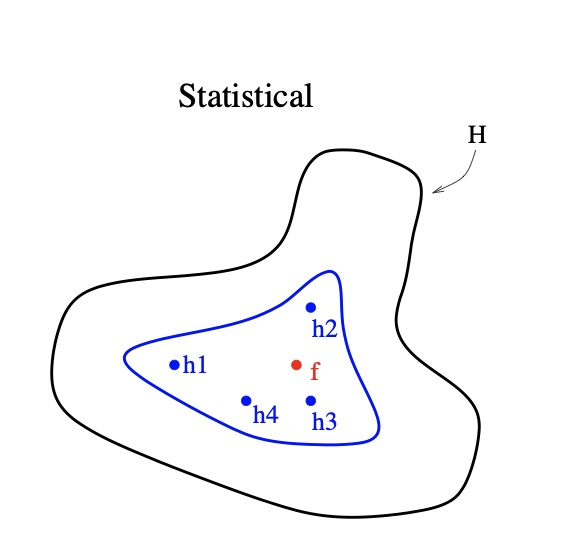
\includegraphics[scale=0.2]{../assets/ensemble/diagrams/statistical.jpg}}
\end{frame}

\begin{frame}{Intuition}
  \pause \textbf{2) Computational:} Some learners are \textit{greedy/non-convex} and can get stuck in local optima.\\
  \pause E.g., decision trees employ greedy splits.

  \vspace{0.5cm}
  \fitpic{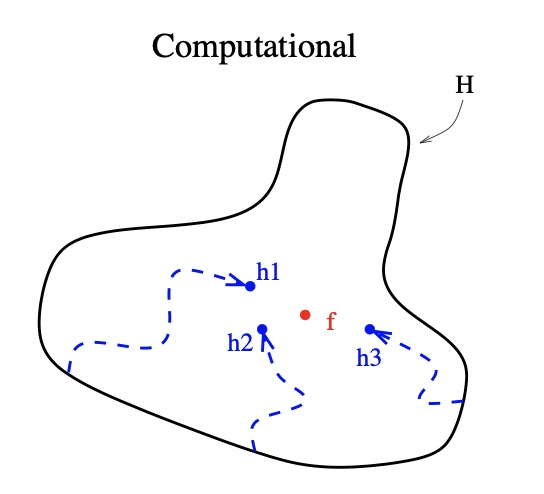
\includegraphics[scale=0.2]{../assets/ensemble/diagrams/computational.jpg}}
\end{frame}

\begin{frame}{Intuition}
  \pause \textbf{3) Representational:} Some models cannot express the true decision boundary.\\
  \pause E.g., axis-parallel splits only (vanilla decision trees).

  \vspace{0.5cm}
  \fitpic{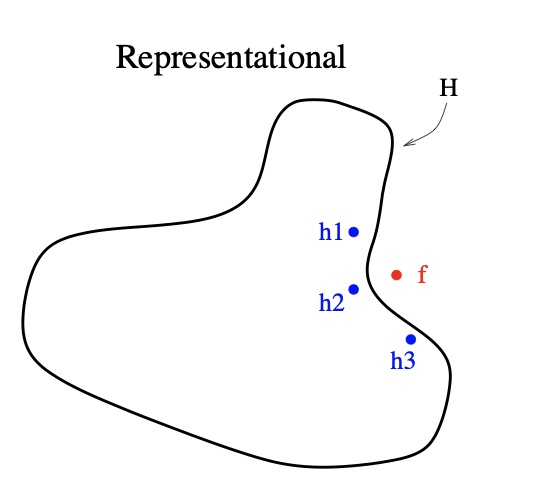
\includegraphics[scale=0.2]{../assets/ensemble/diagrams/representational.jpg}}
\end{frame}

\begin{frame}{Representation of Limited Depth DTs vs RFs}
\begin{figure}[htp]
  \centering
  \begin{notebookbox}{https://nipunbatra.github.io/ml-teaching/notebooks/ensemble-representation.html}
    \fitpic{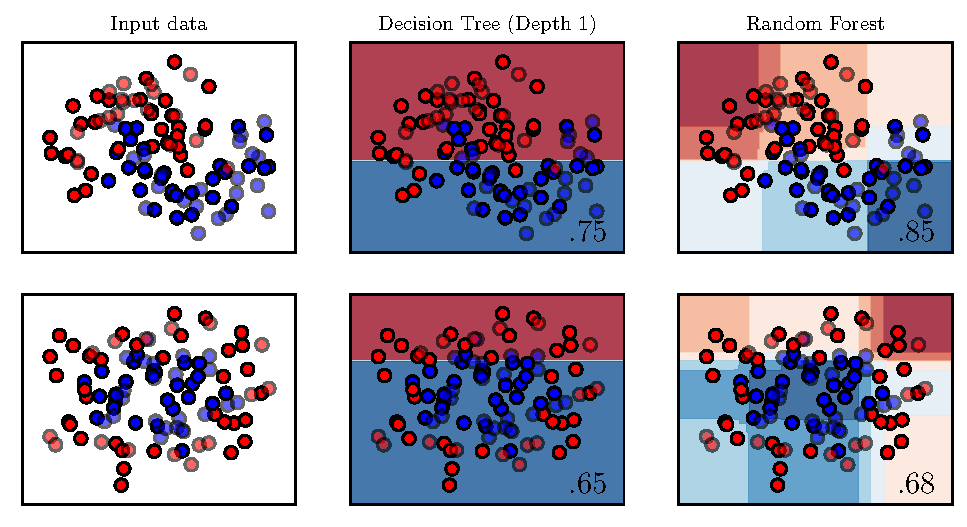
\includegraphics[scale=0.6]{../assets/ensemble/figures/1-representation.pdf}}
  \end{notebookbox}
\end{figure}
\end{frame}

\begin{frame}{Representation of Limited Depth DTs vs RFs}
\begin{figure}[htp]
  \centering
  \begin{notebookbox}{https://nipunbatra.github.io/ml-teaching/notebooks/ensemble-representation.html}
    \fitpic{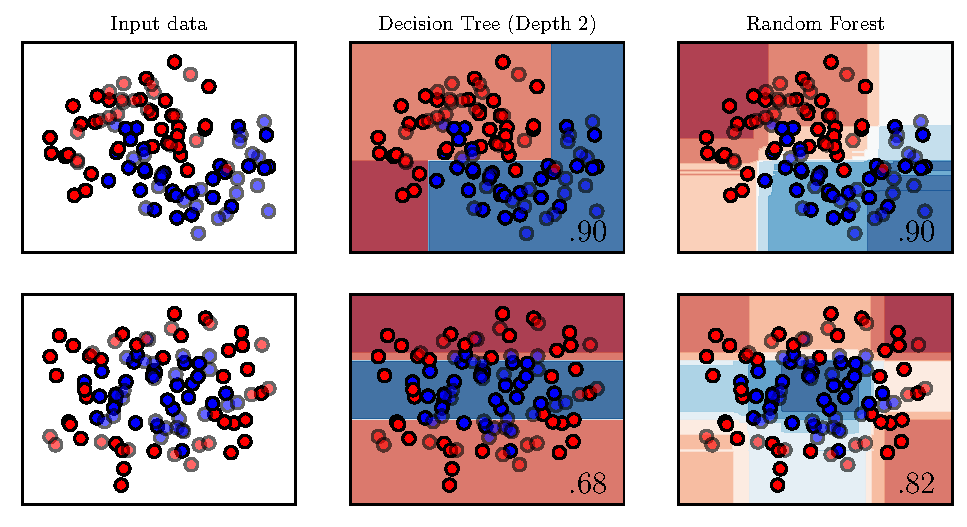
\includegraphics[scale=0.6]{../assets/ensemble/figures/2-representation.pdf}}
  \end{notebookbox}
\end{figure}
\end{frame}

\begin{frame}{Necessary and Sufficient Conditions}
  \small
  \pause 1) A necessary and sufficient condition for an ensemble of classifiers to be more
  accurate than any of its individual members is if the classifiers are \textbf{accurate and
  diverse}.\\[0.4em]

  \pause 2) An \textbf{accurate} classifier \pause is one that has an
  error rate better than random guessing on new $x$ values.\\[0.4em]

  \pause 3) Two classifiers are \textbf{diverse} \pause if they make different errors on new data points.
\end{frame}

\begin{frame}{Necessary and Sufficient Conditions}
  Imagine we have an ensemble of three classifiers ($h_1, h_2, h_3$) and consider a new case $x$.

  \pause If the three classifiers are identical (not diverse),
  when $h_1(x)$ is wrong $h_2(x)$ and $h_3(x)$ will also be wrong.

  \pause If errors are uncorrelated, when $h_1(x)$
  is wrong, $h_2(x)$ and $h_3(x)$ may be correct, so a majority vote correctly
  classifies $x$.
\end{frame}

\begin{frame}{Intuition for Ensembles: Quantitative View}
  \small
  \pause Error probability of each model $\varepsilon=0.3$\\[0.6em]
  $Pr(\text{ensemble wrong}) = \Comb{3}{2}\varepsilon^2(1-\varepsilon)^{1} + \Comb{3}{3}\varepsilon^3(1-\varepsilon)^0
  = 0.19 \le 0.3$
\end{frame}

\begin{frame}{Some calculations}
  \small
  \centering
  \begin{tabular}{c|c|c}
  Number of Models & Ensemble Error & Individual Error \\
  \hline
  1 & 0.3 & 0.3 \\
  3 & 0.216 & 0.3 \\
  5 & 0.163 & 0.3 \\
  \end{tabular}
\end{frame}

\begin{frame}{Some calculations}
  \small
  \centering
  \begin{tabular}{c|c|c}
  Number of Models & Ensemble Error & Individual Error \\
  \hline
  1 & 0.6 & 0.6 \\
  3 & 0.648 & 0.6 \\
  5 & 0.683 & 0.6 \\
  \end{tabular}
\end{frame}

\begin{frame}{Ensemble Methods}
  \only<1->{
    Where does ensemble learning not work well?
  }
  \only<2->{
    \begin{itemize}
      \item The base model is \bad{bad}.
      \item All models make \warn{similar/ correlated} predictions.
    \end{itemize}
  }
\end{frame}

\begin{frame}{Bagging}
  \only<1->{
    Also known as \textbf{Bootstrap Aggregation}.\\
  }
  \only<2->{
    \textbf{Key idea:} Reduce \textbf{variance}.\\
    \vspace{0.6cm}
  }
  \only<3->{
    How to learn different classifiers from the same data?\\[0.2cm]
  }
  \only<4->{
    Think about \textbf{resampling} (cf. cross-validation)!\\[0.2cm]
  }
  \only<5->{
    Create multiple datasets using \textbf{sampling with replacement}.
  }
\end{frame}

\begin{frame}{Bagging}
  \only<1->{
    Dataset with $n$ samples: $D_1,\dots,D_n$.\\
    For each model, create a new dataset of size $n$ by sampling uniformly with replacement.\\
    \vspace{0.6cm}
  }
  \only<2->{
    Round 1: $D_1, D_3, D_6, D_1, \ldots, D_n$\\
    Round 2: $D_2, D_4, D_1, D_{80}, \ldots, D_3$\\
    \vdots
  }
  \only<3->{
    Repetition of samples is possible.\\
  }
  \only<4->{
    Train the same model on each ``bag'' and \textbf{aggregate} predictions.
  }
\end{frame}

\begin{frame}{Bagging : Classification Example}
  Consider the dataset below. Points (3,3) and (5,8) are anomalies.\\[0.3cm]
  \centering
  \fitpic{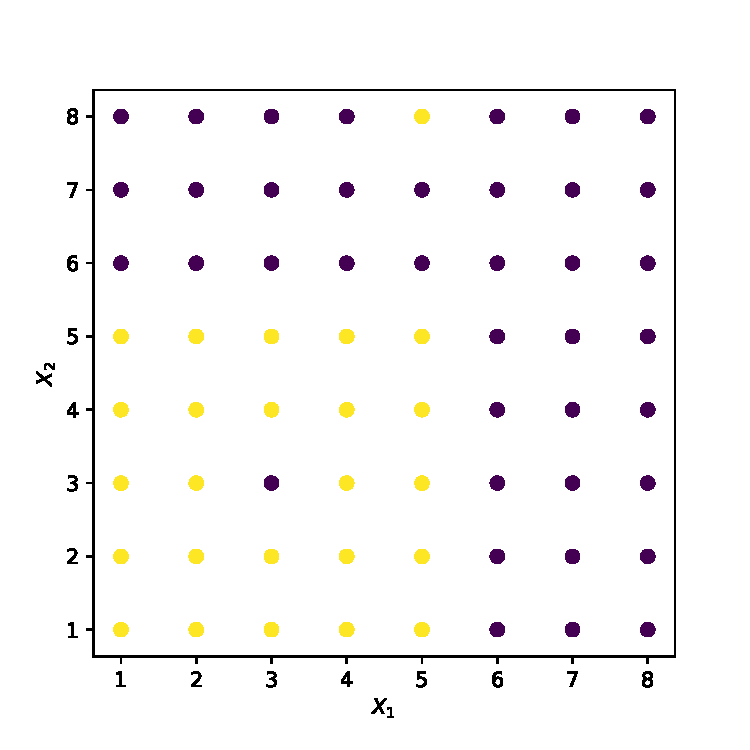
\includegraphics[width=0.6\textwidth]{../assets/ensemble/figures/dataset}}
\end{frame}

\begin{frame}{Bagging : Classification Example}
  Decision Boundary for decision tree with depth 6.\\[0.3cm]
  \centering
  \fitpic{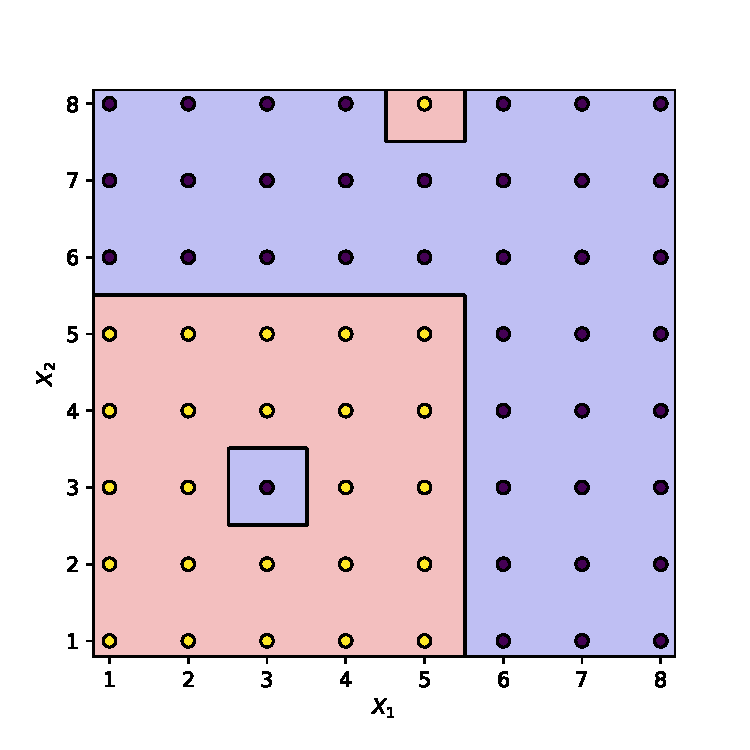
\includegraphics[width=0.6\textwidth]{../assets/ensemble/figures/strong-tree}}
\end{frame}

\begin{frame}{Bagging : Classification Example}
  Let's use bagging with an ensemble of 5 trees.\\[0.3cm]
  \begin{columns}
    \pause\begin{column}{0.33\textwidth}\centering
      Round - 1\\
      \fitpic{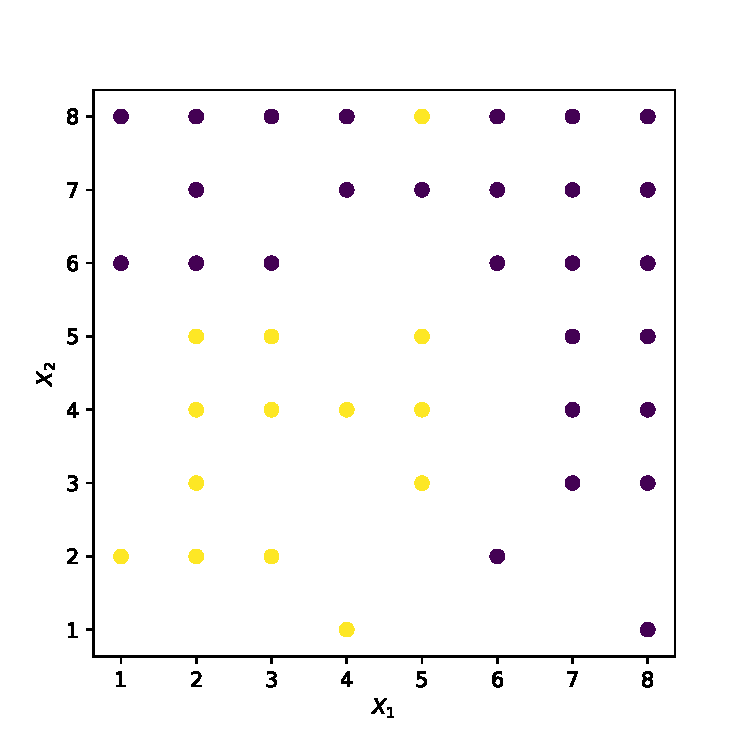
\includegraphics[width=\linewidth]{../assets/ensemble/figures/dataset-rnd-0}}
    \end{column}
    \pause\begin{column}{0.33\textwidth}\centering
      Round - 2\\
      \fitpic{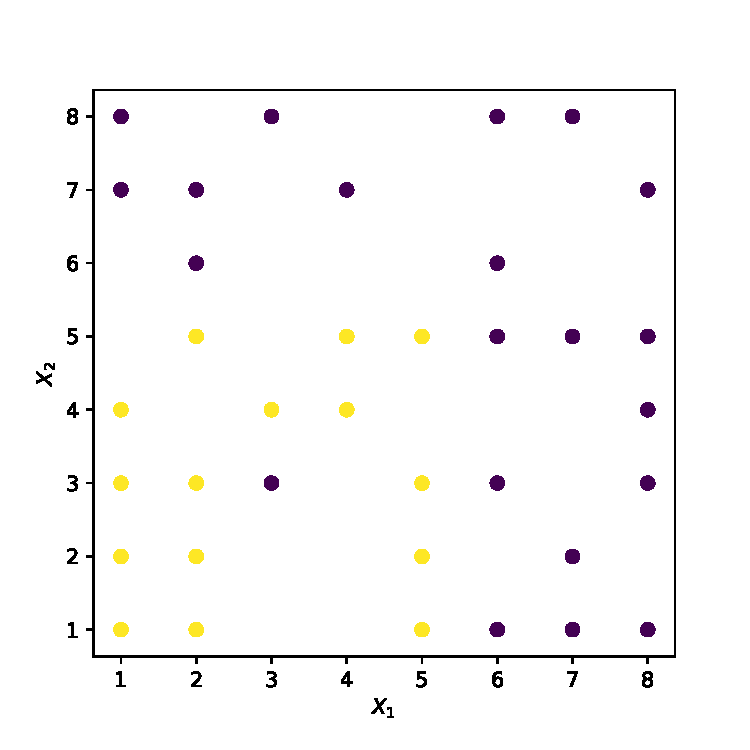
\includegraphics[width=\linewidth]{../assets/ensemble/figures/dataset-rnd-1}}
    \end{column}
    \pause\begin{column}{0.33\textwidth}\centering
      Round - 3\\
      \fitpic{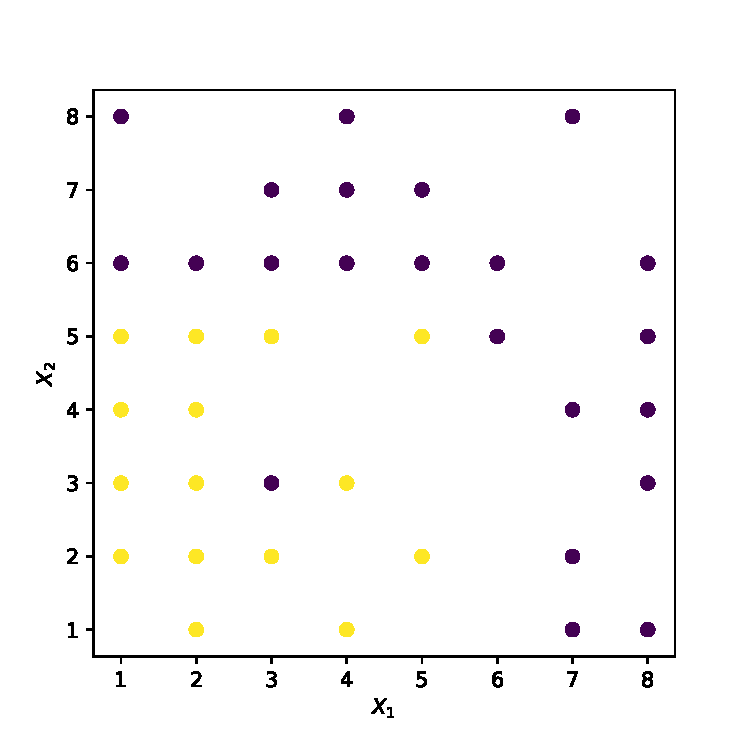
\includegraphics[width=\linewidth]{../assets/ensemble/figures/dataset-rnd-2}}
    \end{column}
  \end{columns}

  \vspace{0.3cm}
  \begin{columns}
    \pause\begin{column}{0.5\textwidth}\centering
      Round - 4\\
      \fitpic{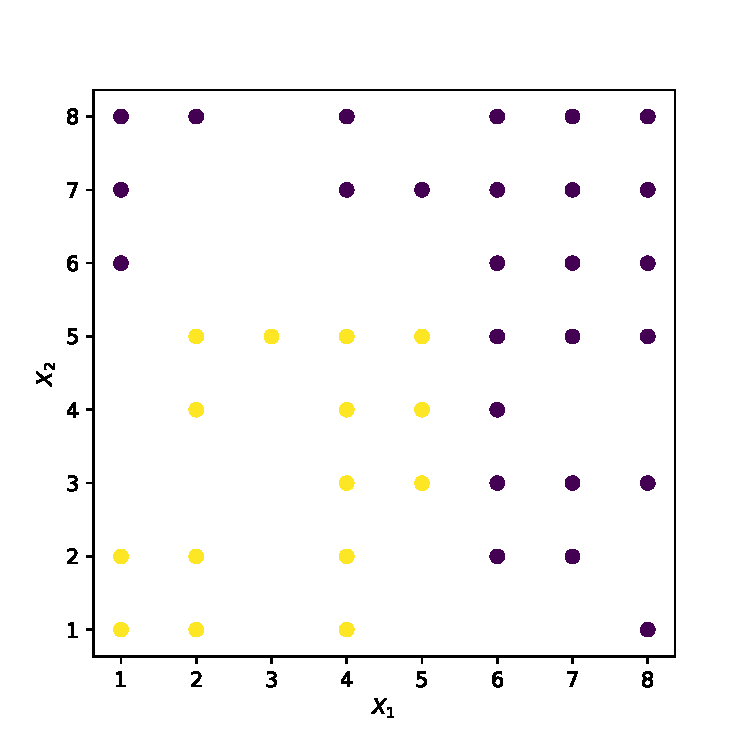
\includegraphics[width=0.9\linewidth]{../assets/ensemble/figures/dataset-rnd-3}}
    \end{column}
    \pause\begin{column}{0.5\textwidth}\centering
      Round - 5\\
      \fitpic{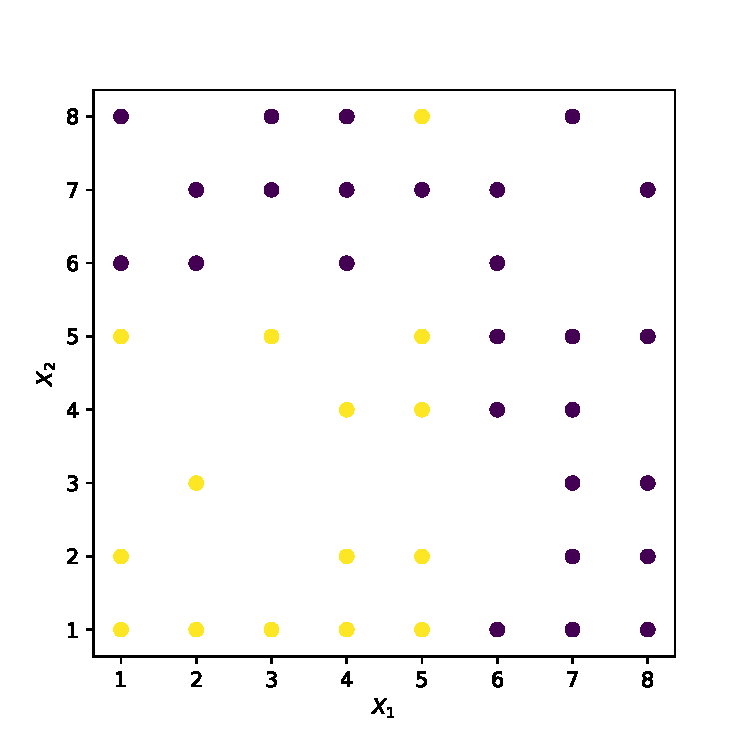
\includegraphics[width=0.9\linewidth]{../assets/ensemble/figures/dataset-rnd-4}}
    \end{column}
  \end{columns}
\end{frame}

\begin{frame}{Bagging : Classification Example}
  \vspace{0.2cm}
  \begin{columns}
    \pause\begin{column}{0.33\textwidth}\centering
      Round - 1\\
      \fitpic{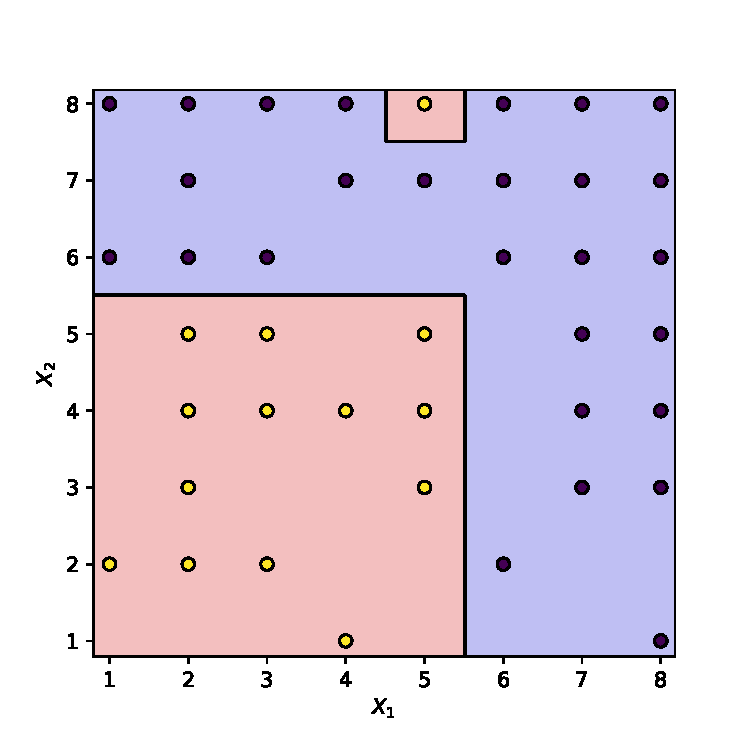
\includegraphics[width=\linewidth]{../assets/ensemble/figures/decision-boundary-0}}\\
      Tree Depth = 4
    \end{column}
    \pause\begin{column}{0.33\textwidth}\centering
      Round - 2\\
      \fitpic{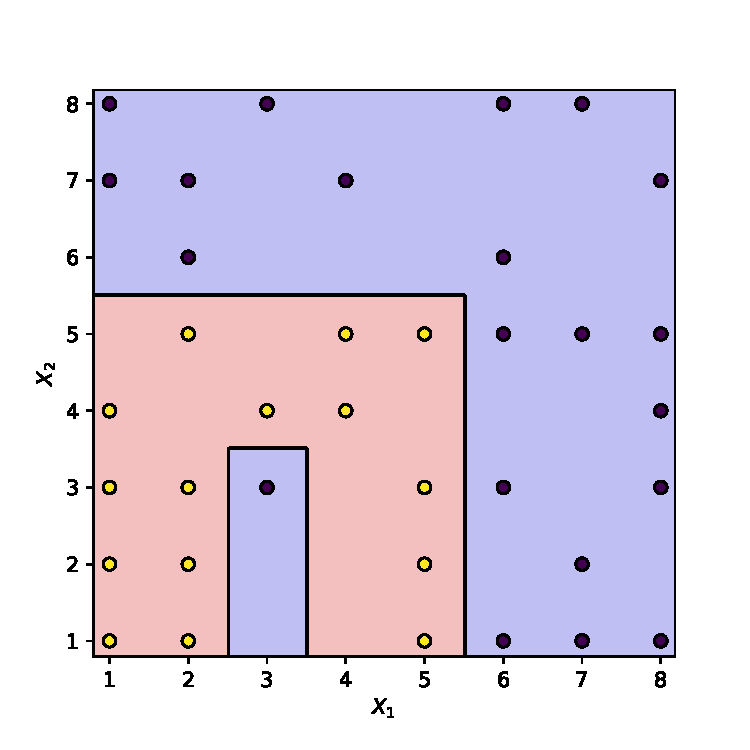
\includegraphics[width=\linewidth]{../assets/ensemble/figures/decision-boundary-1}}\\
      Tree Depth = 5
    \end{column}
    \pause\begin{column}{0.33\textwidth}\centering
      Round - 3\\
      \fitpic{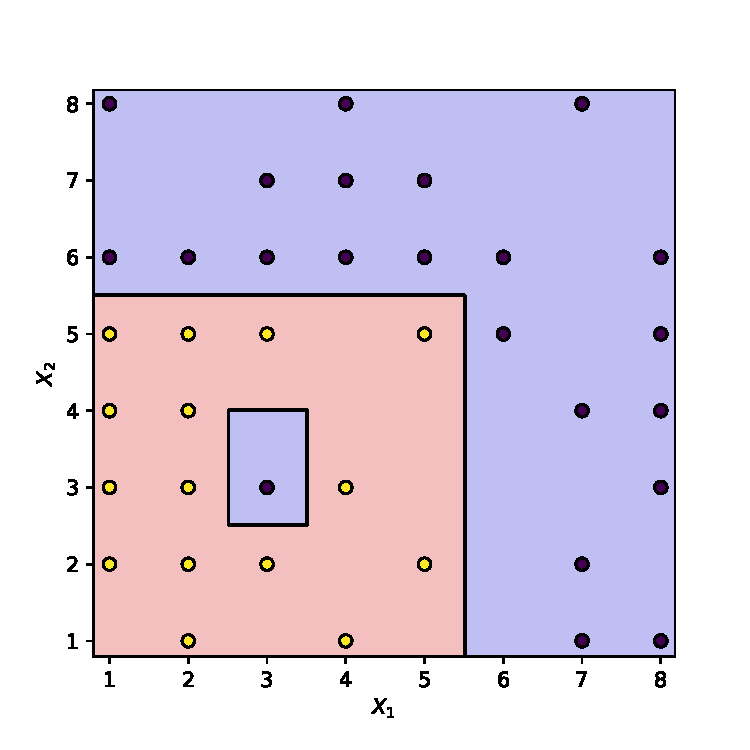
\includegraphics[width=\linewidth]{../assets/ensemble/figures/decision-boundary-2}}\\
      Tree Depth = 5
    \end{column}
  \end{columns}

  \vspace{0.3cm}
  \begin{columns}
    \pause\begin{column}{0.5\textwidth}\centering
      Round - 4\\
      \fitpic{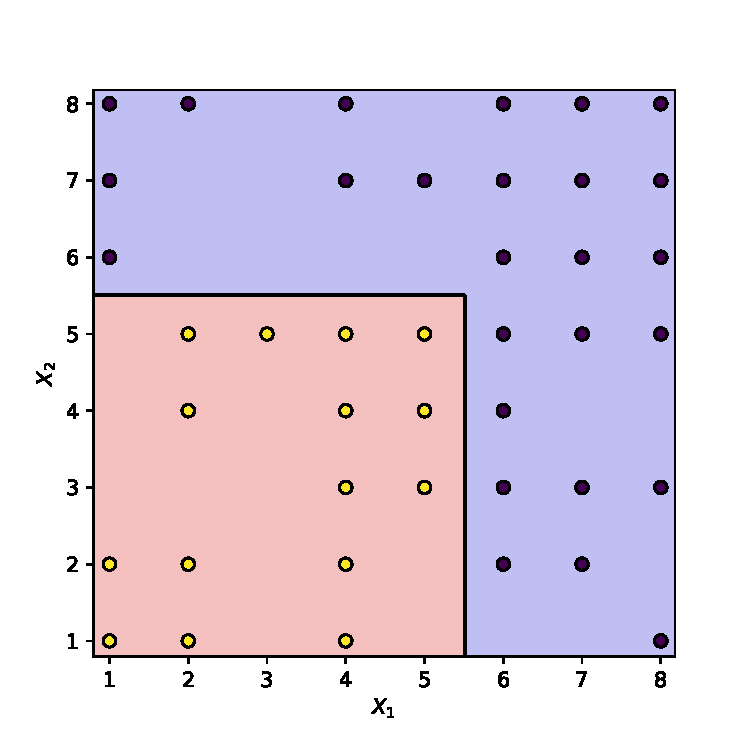
\includegraphics[width=0.9\linewidth]{../assets/ensemble/figures/decision-boundary-3}}\\
      Tree Depth = 2
    \end{column}
    \pause\begin{column}{0.5\textwidth}\centering
      Round - 5\\
      \fitpic{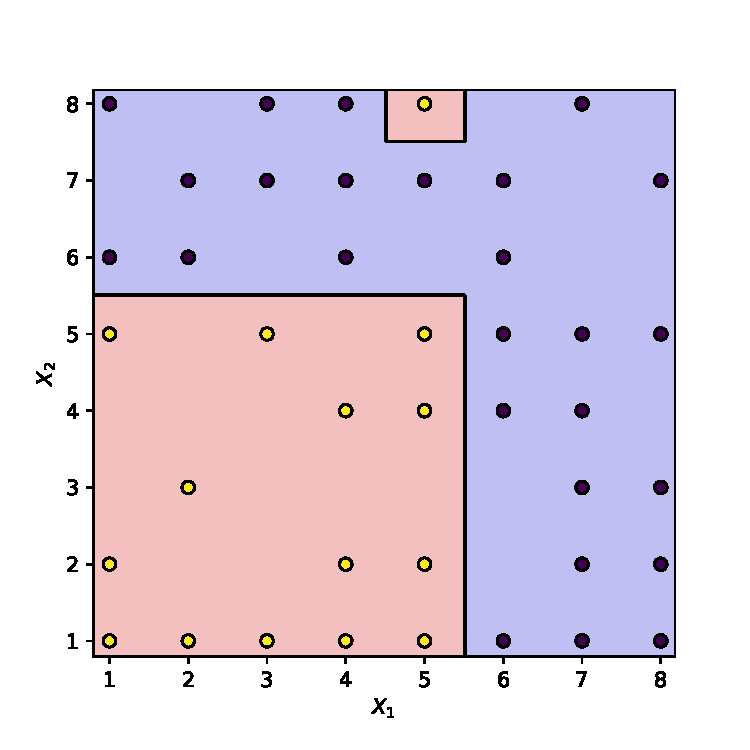
\includegraphics[width=0.9\linewidth]{../assets/ensemble/figures/decision-boundary-4}}\\
      Tree Depth = 4
    \end{column}
  \end{columns}
\end{frame}

\begin{frame}{Bagging : Classification Example}
  Using majority voting to combine all predictions, we get:\\[0.3cm]
  \centering
  \fitpic{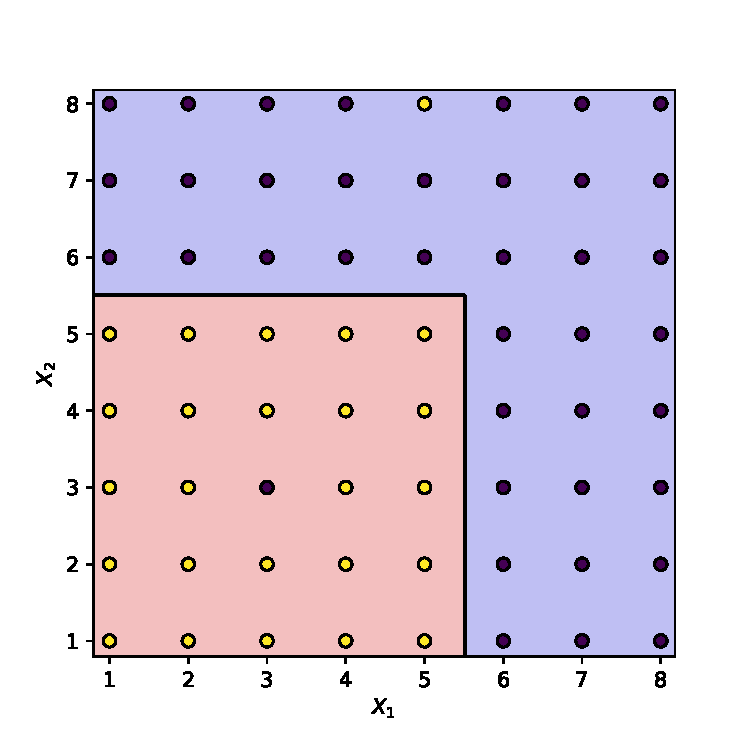
\includegraphics[width=0.6\textwidth]{../assets/ensemble/figures/decision-boundary-ensemble}}
\end{frame}

\begin{frame}{Bagging}
  \textbf{Summary}
  \begin{itemize}
    \item Combine \textbf{strong} learners to reduce \textbf{variance}.
    \item Learners are trained \textbf{independently} on bootstrap samples.
  \end{itemize}
\end{frame}

\begin{frame}{Boosting}
  \begin{itemize}
    \item Combine \textbf{weak} learners to reduce \textbf{bias}.
    \pause \item Learners are built \textbf{incrementally}.
    \pause \item Each round focuses on \textbf{harder} samples (reweighted).
  \end{itemize}
\end{frame}

\begin{frame}{Boosting : AdaBoost }
  Consider a dataset of $N$ samples. Sample $i$ has weight $w_i$. There are $M$ classifiers.\\[0.3cm]
  \centering
  \fitpic{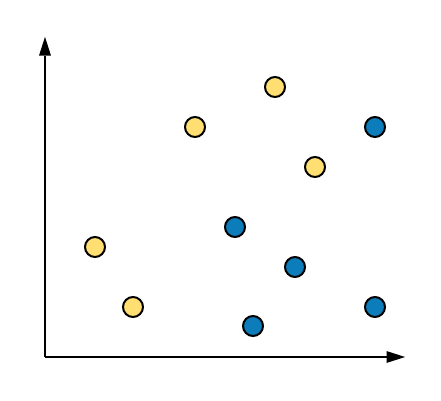
\includegraphics[width=0.6\textwidth]{../assets/ensemble/diagrams/ada_data}}
\end{frame}

\begin{frame}{Boosting : AdaBoost }
  Consider a dataset of $N$ samples. Sample $i$ has weight $w_i$. There are $M$ classifiers.\\[0.3cm]
  \begin{enumerate}
    \item Initialize weights: $w_i = \frac{1}{N}$
  \end{enumerate}
  \centering
  \fitpic{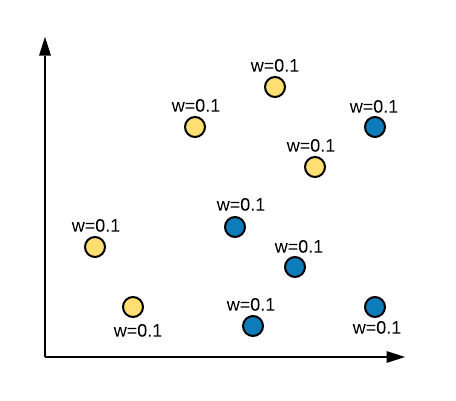
\includegraphics[width=0.6\textwidth]{../assets/ensemble/diagrams/ada_data_init_weights}}
\end{frame}

\begin{frame}{Boosting : AdaBoost }
  Consider a dataset of $N$ samples. Sample $i$ has weight $w_i$. There are $M$ classifiers.\\[0.3cm]
  \begin{enumerate}
    \item Initialize weights: $w_i = \frac{1}{N}$
    \item For $m = 1, \ldots, M$:
          \begin{enumerate}
            \item Learn classifier using current weights $w_i$
          \end{enumerate}
  \end{enumerate}
  \centering
  \fitpic{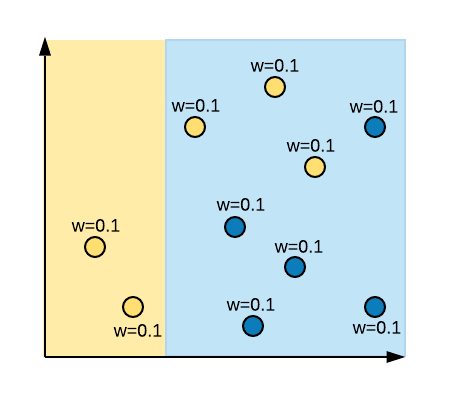
\includegraphics[width=0.85\textwidth]{../assets/ensemble/diagrams/ada_iter1}}
\end{frame}

\begin{frame}{Boosting : AdaBoost }
  Consider a dataset of $N$ samples. Sample $i$ has weight $w_i$. There are $M$ classifiers.\\[0.3cm]
  \begin{enumerate}
    \item Initialize weights: $w_i = \frac{1}{N}$
    \item For $m = 1, \ldots, M$:
          \begin{enumerate}
            \item Learn classifier using current weights $w_i$
          \end{enumerate}
  \end{enumerate}
  \centering
  \fitpic{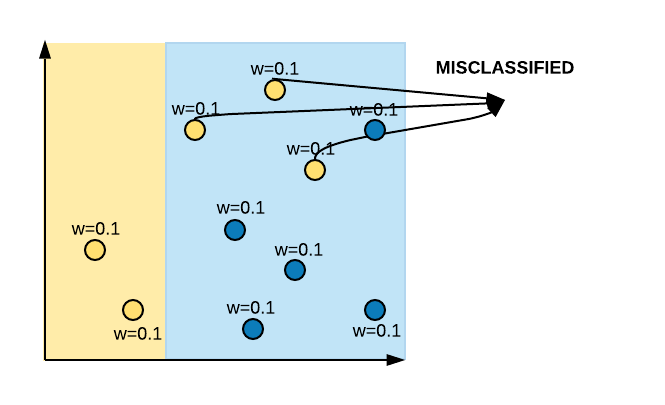
\includegraphics[width=0.85\textwidth]{../assets/ensemble/diagrams/ada_iter1_misclassify}}
\end{frame}

\begin{frame}{Boosting : AdaBoost }
  Consider a dataset of $N$ samples. Sample $i$ has weight $w_i$. There are $M$ classifiers.\\[0.3cm]
  \begin{enumerate}
    \item Initialize weights: $w_i = \frac{1}{N}$
    \item For $m = 1, \ldots, M$:
          \begin{enumerate}
            \item Learn classifier using current weights $w_i$
            \item Compute weighted error: $\text{err}_m = \frac{\sum_i w_i(\text{incorrect})}{\sum_i w_i}$
          \end{enumerate}
  \end{enumerate}
  \begin{columns}
    \begin{column}{0.5\textwidth}\centering
      \fitpic{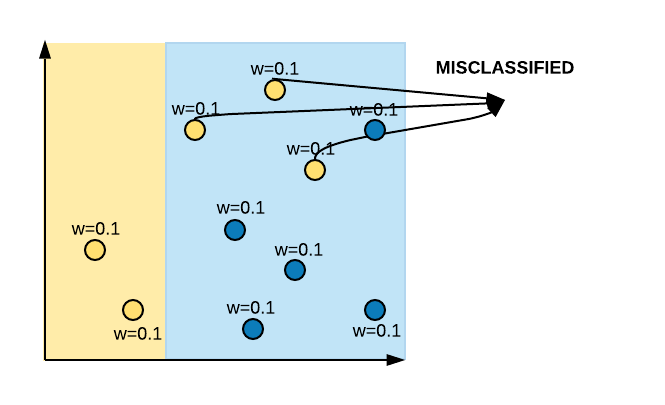
\includegraphics[width=1.1\textwidth]{../assets/ensemble/diagrams/ada_iter1_misclassify}}
    \end{column}
    \begin{column}{0.5\textwidth}
      $err_1 = \dfrac{0.3}{1}$
    \end{column}
  \end{columns}
\end{frame}

\begin{frame}{Boosting : AdaBoost }
  Consider a dataset of $N$ samples. Sample $i$ has weight $w_i$. There are $M$ classifiers.\\[0.3cm]
  \begin{enumerate}
    \item Initialize weights: $w_i = \frac{1}{N}$
    \item For $m = 1, \ldots, M$:
          \begin{enumerate}
            \item Learn classifier using current weights $w_i$
            \item Compute weighted error: $\text{err}_m = \frac{\sum_i w_i(\text{incorrect})}{\sum_i w_i}$
            \item Compute $\alpha_m = \tfrac{1}{2}\log\!\left(\frac{1 - \text{err}_m}{\text{err}_m}\right)$
          \end{enumerate}
  \end{enumerate}
  \begin{columns}
    \begin{column}{0.5\textwidth}\centering
      \fitpic{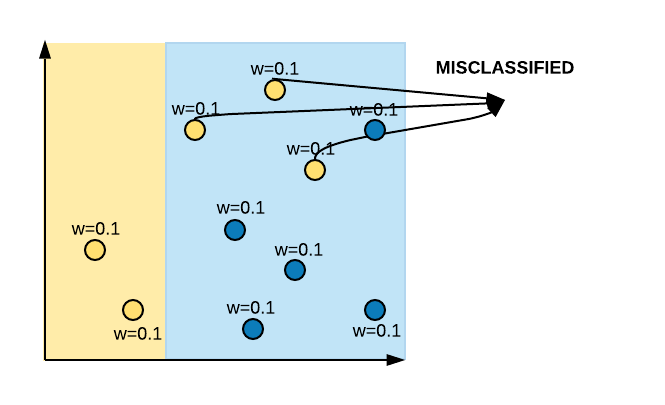
\includegraphics[width=\textwidth]{../assets/ensemble/diagrams/ada_iter1_misclassify}}
    \end{column}
    \begin{column}{0.5\textwidth}
      $err_1 = 0.3$\\
      $\alpha_1 = \tfrac{1}{2}\log\!\left(\frac{0.7}{0.3}\right) \approx 0.42$
    \end{column}
  \end{columns}
\end{frame}

\begin{frame}{Boosting : AdaBoost }
  Consider a dataset of $N$ samples. Sample $i$ has weight $w_i$. There are $M$ classifiers.\\[0.3cm]
  \begin{enumerate}
    \item Initialize weights: $w_i = \frac{1}{N}$
    \item For $m = 1, \ldots, M$:
          \begin{enumerate}
            \item Learn classifier using current weights $w_i$
            \item Compute weighted error: $\text{err}_m = \frac{\sum_i w_i(\text{incorrect})}{\sum_i w_i}$
            \item Compute $\alpha_m = \tfrac{1}{2}\log\!\left(\frac{1 - \text{err}_m}{\text{err}_m}\right)$
            \item If correct: $w_i \leftarrow w_i e^{-\alpha_m}$ \quad If incorrect: $w_i \leftarrow w_i e^{\alpha_m}$
          \end{enumerate}
  \end{enumerate}
\end{frame}

\begin{frame}{Boosting : AdaBoost }
  \centering
  \fitpic{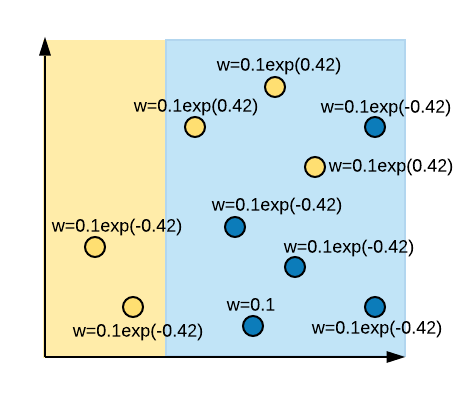
\includegraphics[width=0.8\textwidth]{../assets/ensemble/diagrams/ada_iter1_new_weights_exp}}
\end{frame}

\begin{frame}{Boosting : AdaBoost }
  \centering
  \fitpic{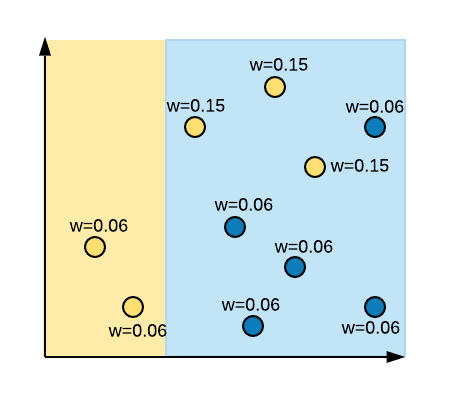
\includegraphics[width=0.8\textwidth]{../assets/ensemble/diagrams/ada_iter1_new_weights}}
\end{frame}

\begin{frame}{Boosting : AdaBoost }
  Consider a dataset of $N$ samples. Sample $i$ has weight $w_i$. There are $M$ classifiers.\\[0.3cm]
  \begin{enumerate}
    \item Initialize weights: $w_i = \frac{1}{N}$
    \item For $m = 1, \ldots, M$:
          \begin{enumerate}
            \item Learn classifier using current weights $w_i$
            \item Compute weighted error: $\text{err}_m = \frac{\sum_i w_i(\text{incorrect})}{\sum_i w_i}$
            \item Compute $\alpha_m = \tfrac{1}{2}\log\!\left(\frac{1 - \text{err}_m}{\text{err}_m}\right)$
            \item Update $w_i$ as above
            \item Normalize $w_i$ to sum to 1
          \end{enumerate}
  \end{enumerate}
\end{frame}

\begin{frame}{Boosting : AdaBoost }
  \centering
  \fitpic{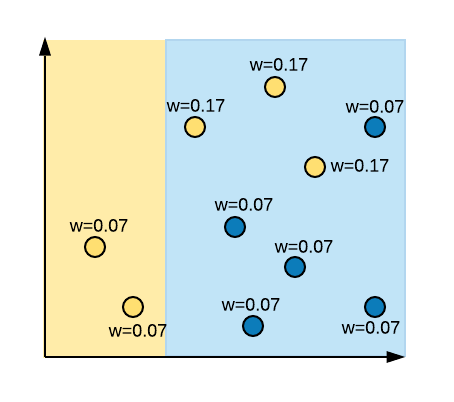
\includegraphics[width=0.8\textwidth]{../assets/ensemble/diagrams/ada_iter1_new_weights_normalized}}
\end{frame}

\begin{frame}{Boosting : AdaBoost }
  Consider a dataset of $N$ samples. Sample $i$ has weight $w_i$. There are $M$ classifiers.\\[0.3cm]
  \begin{enumerate}
    \item Initialize weights: $w_i = \frac{1}{N}$
    \item For $m = 1, \ldots, M$:
          \begin{enumerate}
            \item Learn classifier using current weights $w_i$
            \item Compute weighted error: $\text{err}_m = \frac{\sum_i w_i(\text{incorrect})}{\sum_i w_i}$
            \item Compute $\alpha_m = \tfrac{1}{2}\log\!\left(\frac{1 - \text{err}_m}{\text{err}_m}\right)$
          \end{enumerate}
  \end{enumerate}
  \begin{columns}
    \begin{column}{0.5\textwidth}\centering
      \fitpic{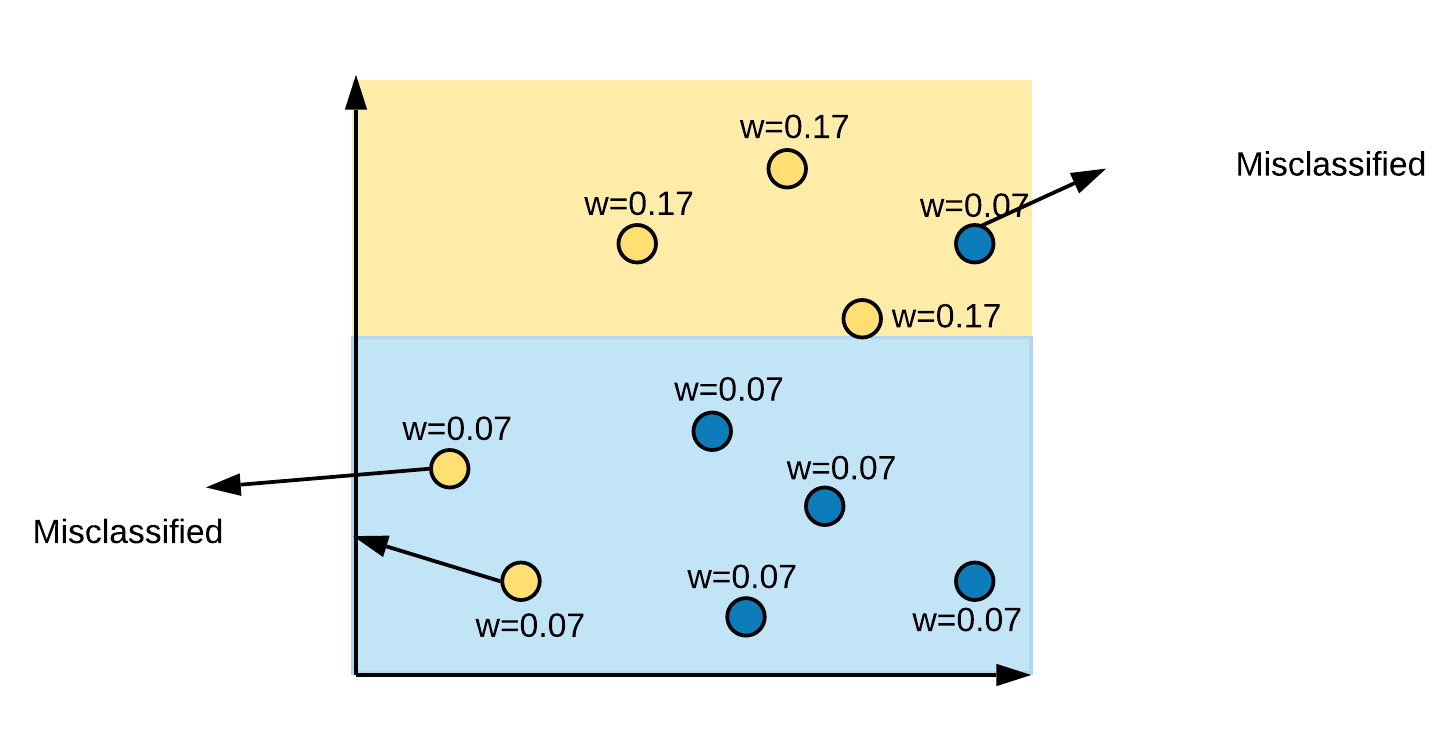
\includegraphics[width=\textwidth]{../assets/ensemble/diagrams/ada_iter2_misclassify}}
    \end{column}
    \begin{column}{0.5\textwidth}
      $err_2 = 0.21$\\
      $\alpha_2 = \tfrac{1}{2}\log\!\left(\frac{0.79}{0.21}\right) \approx 0.66$
    \end{column}
  \end{columns}
\end{frame}

\begin{frame}{Boosting : AdaBoost }
  \centering
  \fitpic{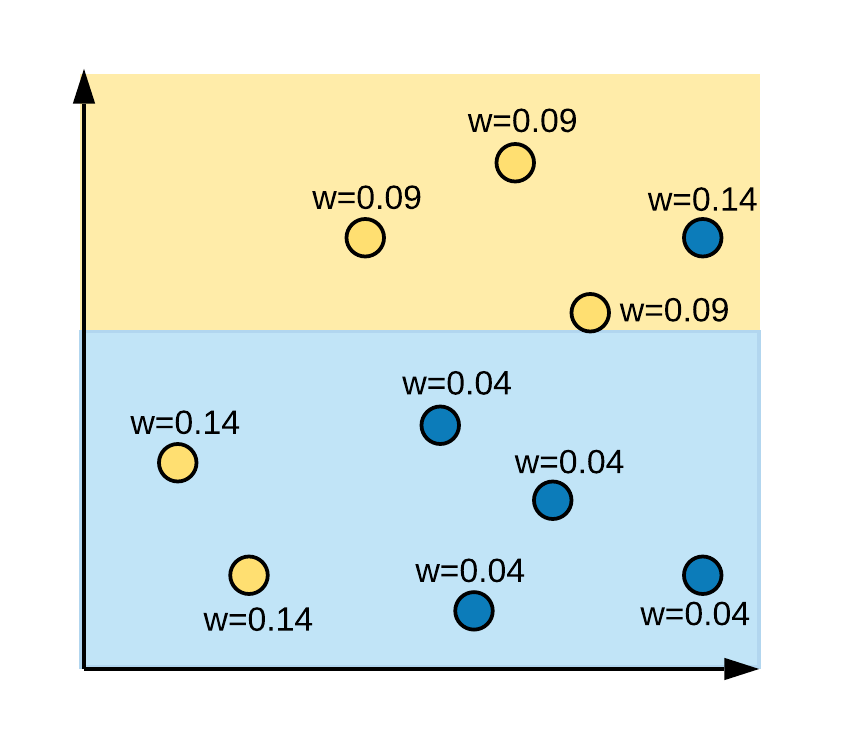
\includegraphics[width=0.8\textwidth]{../assets/ensemble/diagrams/ada_iter2_new_weights}}
\end{frame}

\begin{frame}{Boosting : AdaBoost }
  Consider a dataset of $N$ samples. Sample $i$ has weight $w_i$. There are $M$ classifiers.\\[0.3cm]
  \begin{enumerate}
    \item Initialize weights: $w_i = \frac{1}{N}$
    \item For $m = 1, \ldots, M$:
          \begin{enumerate}
            \item Learn classifier using current weights $w_i$
            \item Compute weighted error: $\text{err}_m = \frac{\sum_i w_i(\text{incorrect})}{\sum_i w_i}$
            \item Compute $\alpha_m = \tfrac{1}{2}\log\!\left(\frac{1 - \text{err}_m}{\text{err}_m}\right)$
            \item Update $w_i$ as above
          \end{enumerate}
  \end{enumerate}
\end{frame}

\begin{frame}{Boosting : AdaBoost }
  \centering
  \fitpic{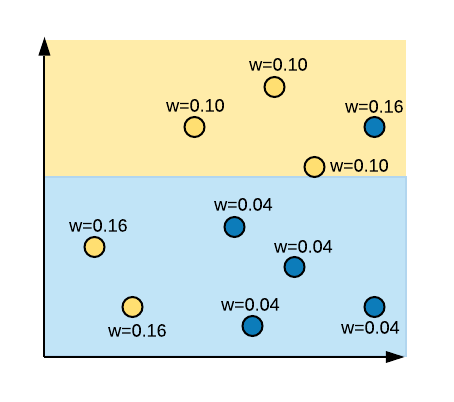
\includegraphics[width=0.8\textwidth]{../assets/ensemble/diagrams/ada_iter2_new_weights_normalized}}
\end{frame}

\begin{frame}{Boosting : AdaBoost }
  Consider a dataset of $N$ samples. Sample $i$ has weight $w_i$. There are $M$ classifiers.\\[0.3cm]
  \begin{enumerate}
    \item Initialize weights: $w_i = \frac{1}{N}$
    \item For $m = 1, \ldots, M$:
          \begin{enumerate}
            \item Learn classifier using current weights $w_i$
            \item Compute weighted error: $\text{err}_m = \frac{\sum_i w_i(\text{incorrect})}{\sum_i w_i}$
            \item Compute $\alpha_m = \tfrac{1}{2}\log\!\left(\frac{1 - \text{err}_m}{\text{err}_m}\right)$
          \end{enumerate}
  \end{enumerate}
  \begin{columns}
    \begin{column}{0.5\textwidth}\centering
      \fitpic{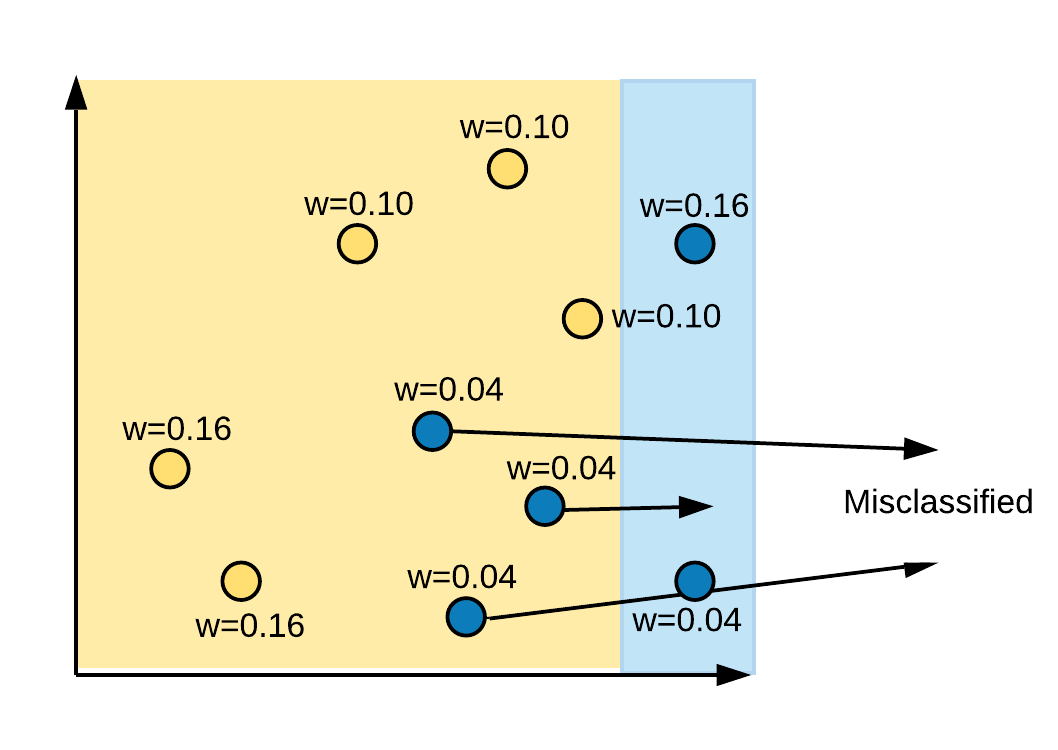
\includegraphics[width=\textwidth]{../assets/ensemble/diagrams/ada_iter3_misclassify}}
    \end{column}
    \begin{column}{0.5\textwidth}
      $err_3 = 0.12$\\
      $\alpha_3 = \tfrac{1}{2}\log\!\left(\frac{0.88}{0.12}\right) \approx 0.99$
    \end{column}
  \end{columns}
\end{frame}

\begin{frame}{Boosting: AdaBoost}
  \small
  \textbf{Intuition:} after each iteration, importance of wrongly classified samples increases (weights up), and importance of correctly classified samples decreases (weights down).
\end{frame}

\begin{frame}{Boosting: AdaBoost}
  \textbf{Testing}\\[0.2cm]
  \begin{itemize}
    \item For each sample $x$, compute $h_m(x)$ for all $m$.
    \item Final prediction: \(\mathrm{sign}\!\left(\alpha_1 h_1(x)+\alpha_2 h_2(x)+\cdots+\alpha_M h_M(x)\right)\).
  \end{itemize}
\end{frame}

\begin{frame}{Boosting: AdaBoost}
  \textbf{Example}
  \begin{columns}
    \pause\begin{column}{0.33\textwidth}\centering
      \fitpic{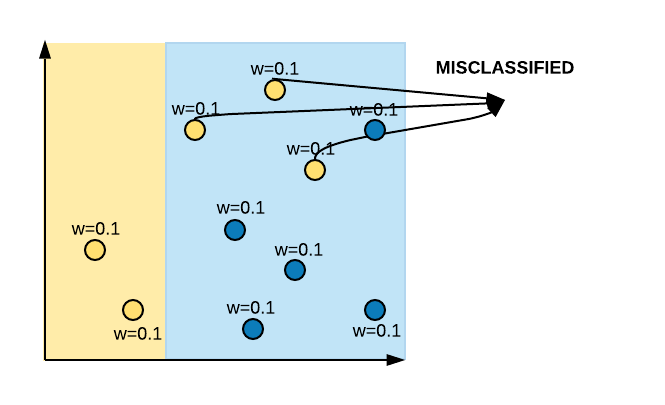
\includegraphics[width=\linewidth]{../assets/ensemble/diagrams/ada_iter1_misclassify}}
      \vspace{-8pt}\captionof{figure}{$\alpha_1=0.42$}
    \end{column}
    \pause\begin{column}{0.33\textwidth}\centering
      \fitpic{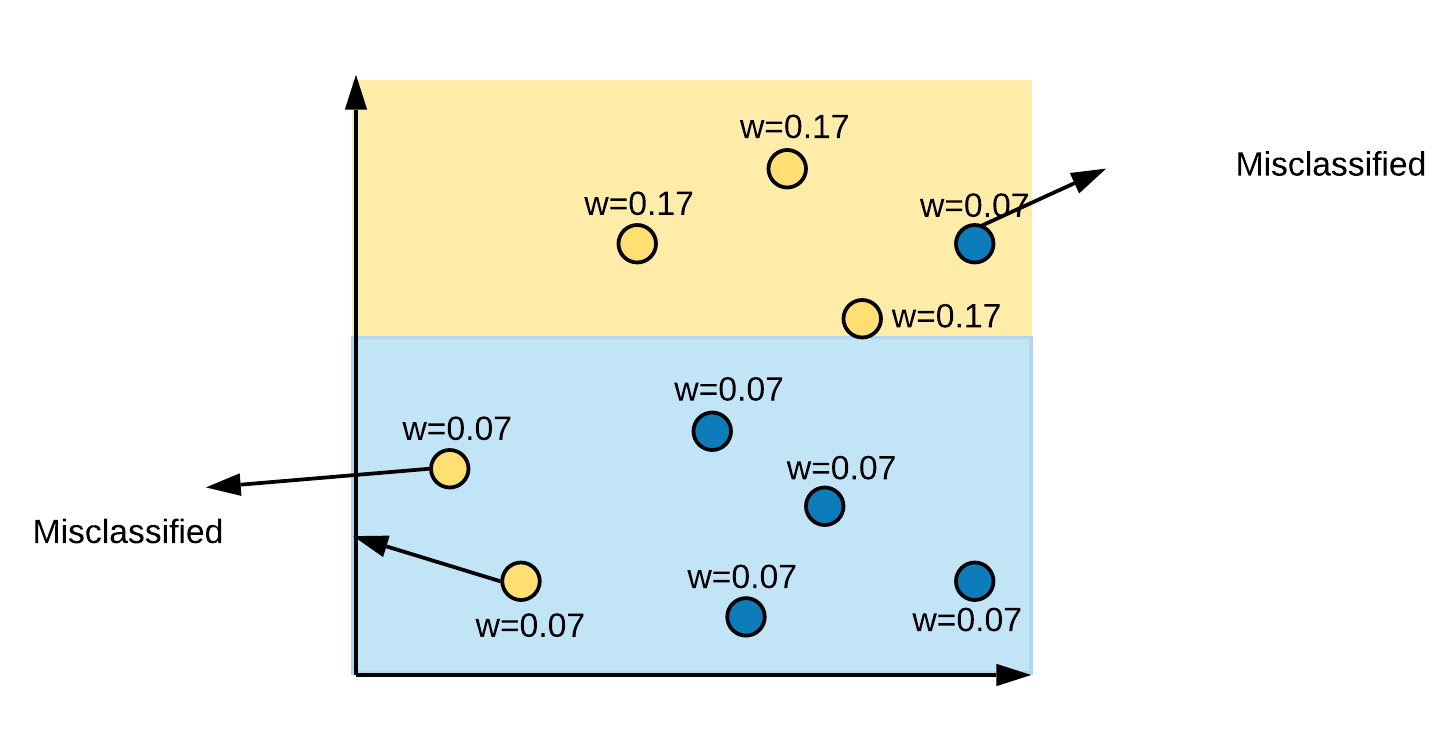
\includegraphics[width=\linewidth]{../assets/ensemble/diagrams/ada_iter2_misclassify}}
      \vspace{-8pt}\captionof{figure}{$\alpha_2=0.66$}
    \end{column}
    \pause\begin{column}{0.33\textwidth}\centering
      \fitpic{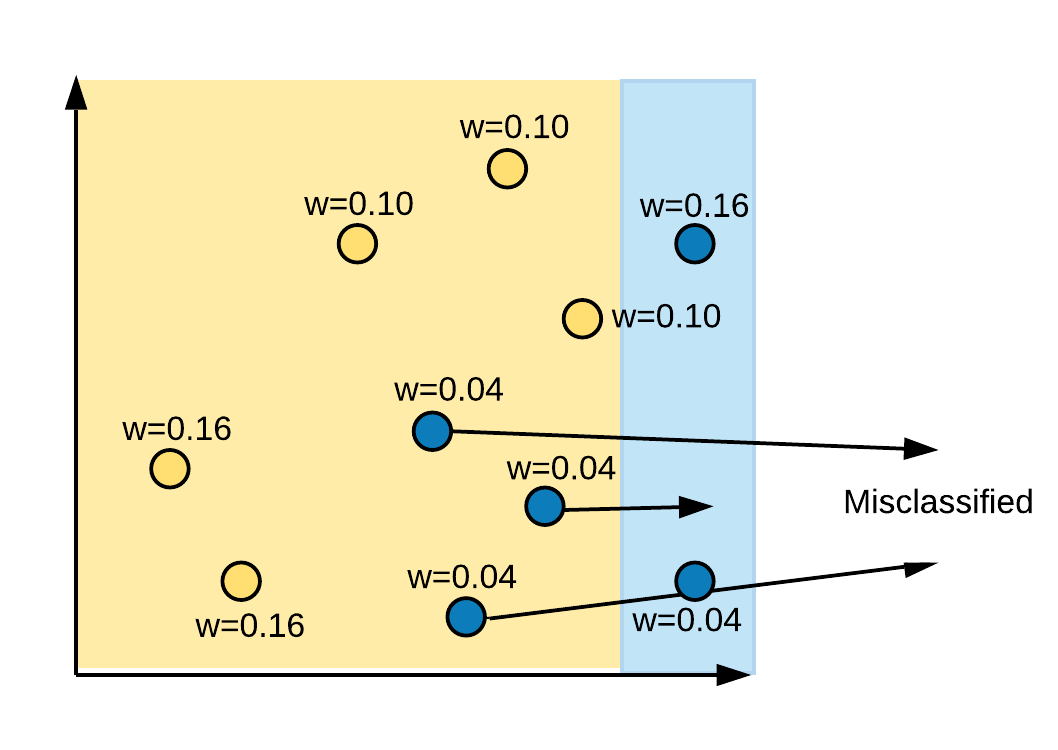
\includegraphics[width=\linewidth]{../assets/ensemble/diagrams/ada_iter3_misclassify}}
      \vspace{-8pt}\captionof{figure}{$\alpha_3=0.99$}
    \end{column}
  \end{columns}

  \vspace{0.3cm}
  \begin{columns}
    \pause\begin{column}{0.5\textwidth}\centering
      \fitpic{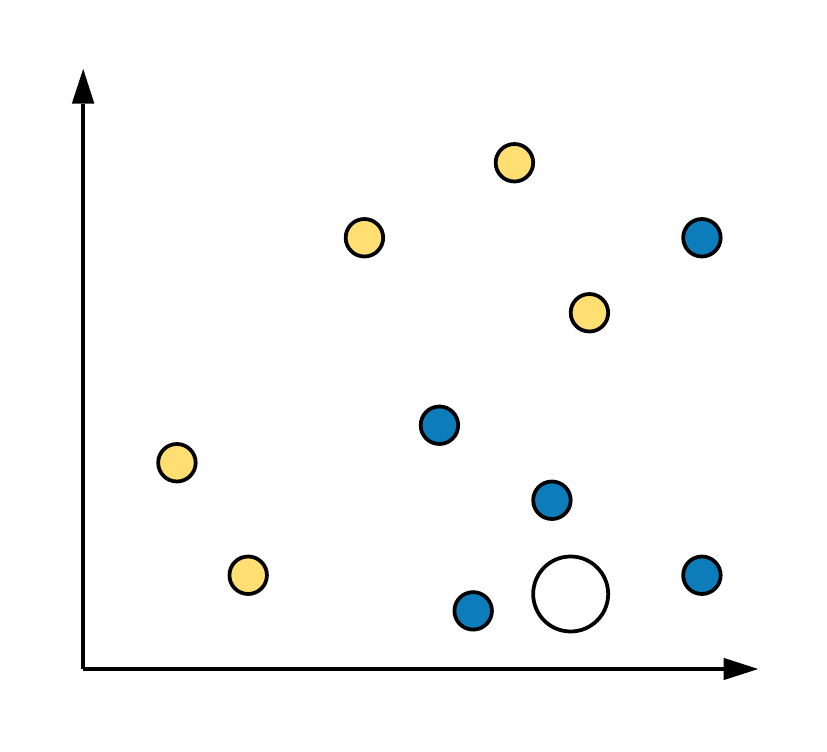
\includegraphics[scale=0.1]{../assets/ensemble/diagrams/testing}}
    \end{column}
    \begin{column}{0.5\textwidth}
      \pause Let yellow be $+1$ and blue be $-1$.\\[0.3em]
      \pause Prediction $= \mathrm{sign}(0.42\cdot{-1} + 0.66\cdot{-1} + 0.99\cdot{+1}) = \text{Negative (blue)}$.
    \end{column}
  \end{columns}
\end{frame}

\begin{frame}{Intuition behind weight update formula}
  \begin{columns}
    \pause\begin{column}{0.5\textwidth}
      \begin{figure}[htp]\centering
        \begin{notebookbox}{https://nipunbatra.github.io/ml-teaching/notebooks/boosting-explanation.html}
          \fitpic{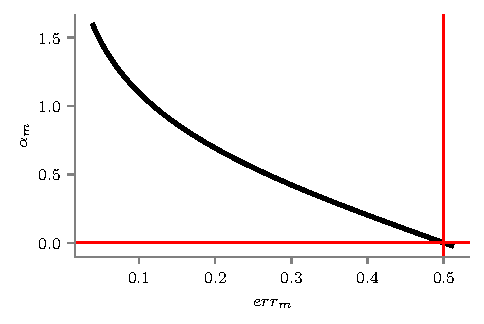
\includegraphics[scale=0.55]{../assets/ensemble/figures/alpha-boosting.pdf}}
        \end{notebookbox}
      \end{figure}
    \end{column}
    \pause\begin{column}{0.5\textwidth}
      \begin{figure}[htp]\centering
        \begin{notebookbox}{https://nipunbatra.github.io/ml-teaching/notebooks/boosting-explanation.html}
          \fitpic{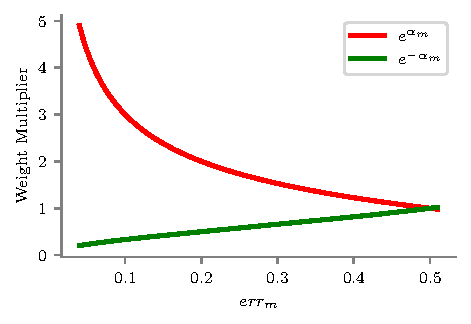
\includegraphics[scale=0.55]{../assets/ensemble/figures/alpha-boosting-weight.pdf}}
        \end{notebookbox}
      \end{figure}
    \end{column}
  \end{columns}
\end{frame}

\begin{frame}{AdaBoost for Regression}
  From paper: \emph{Improving Regressors using Boosting Techniques}
  \vspace{0.3cm}

  \centering
  \fitpic{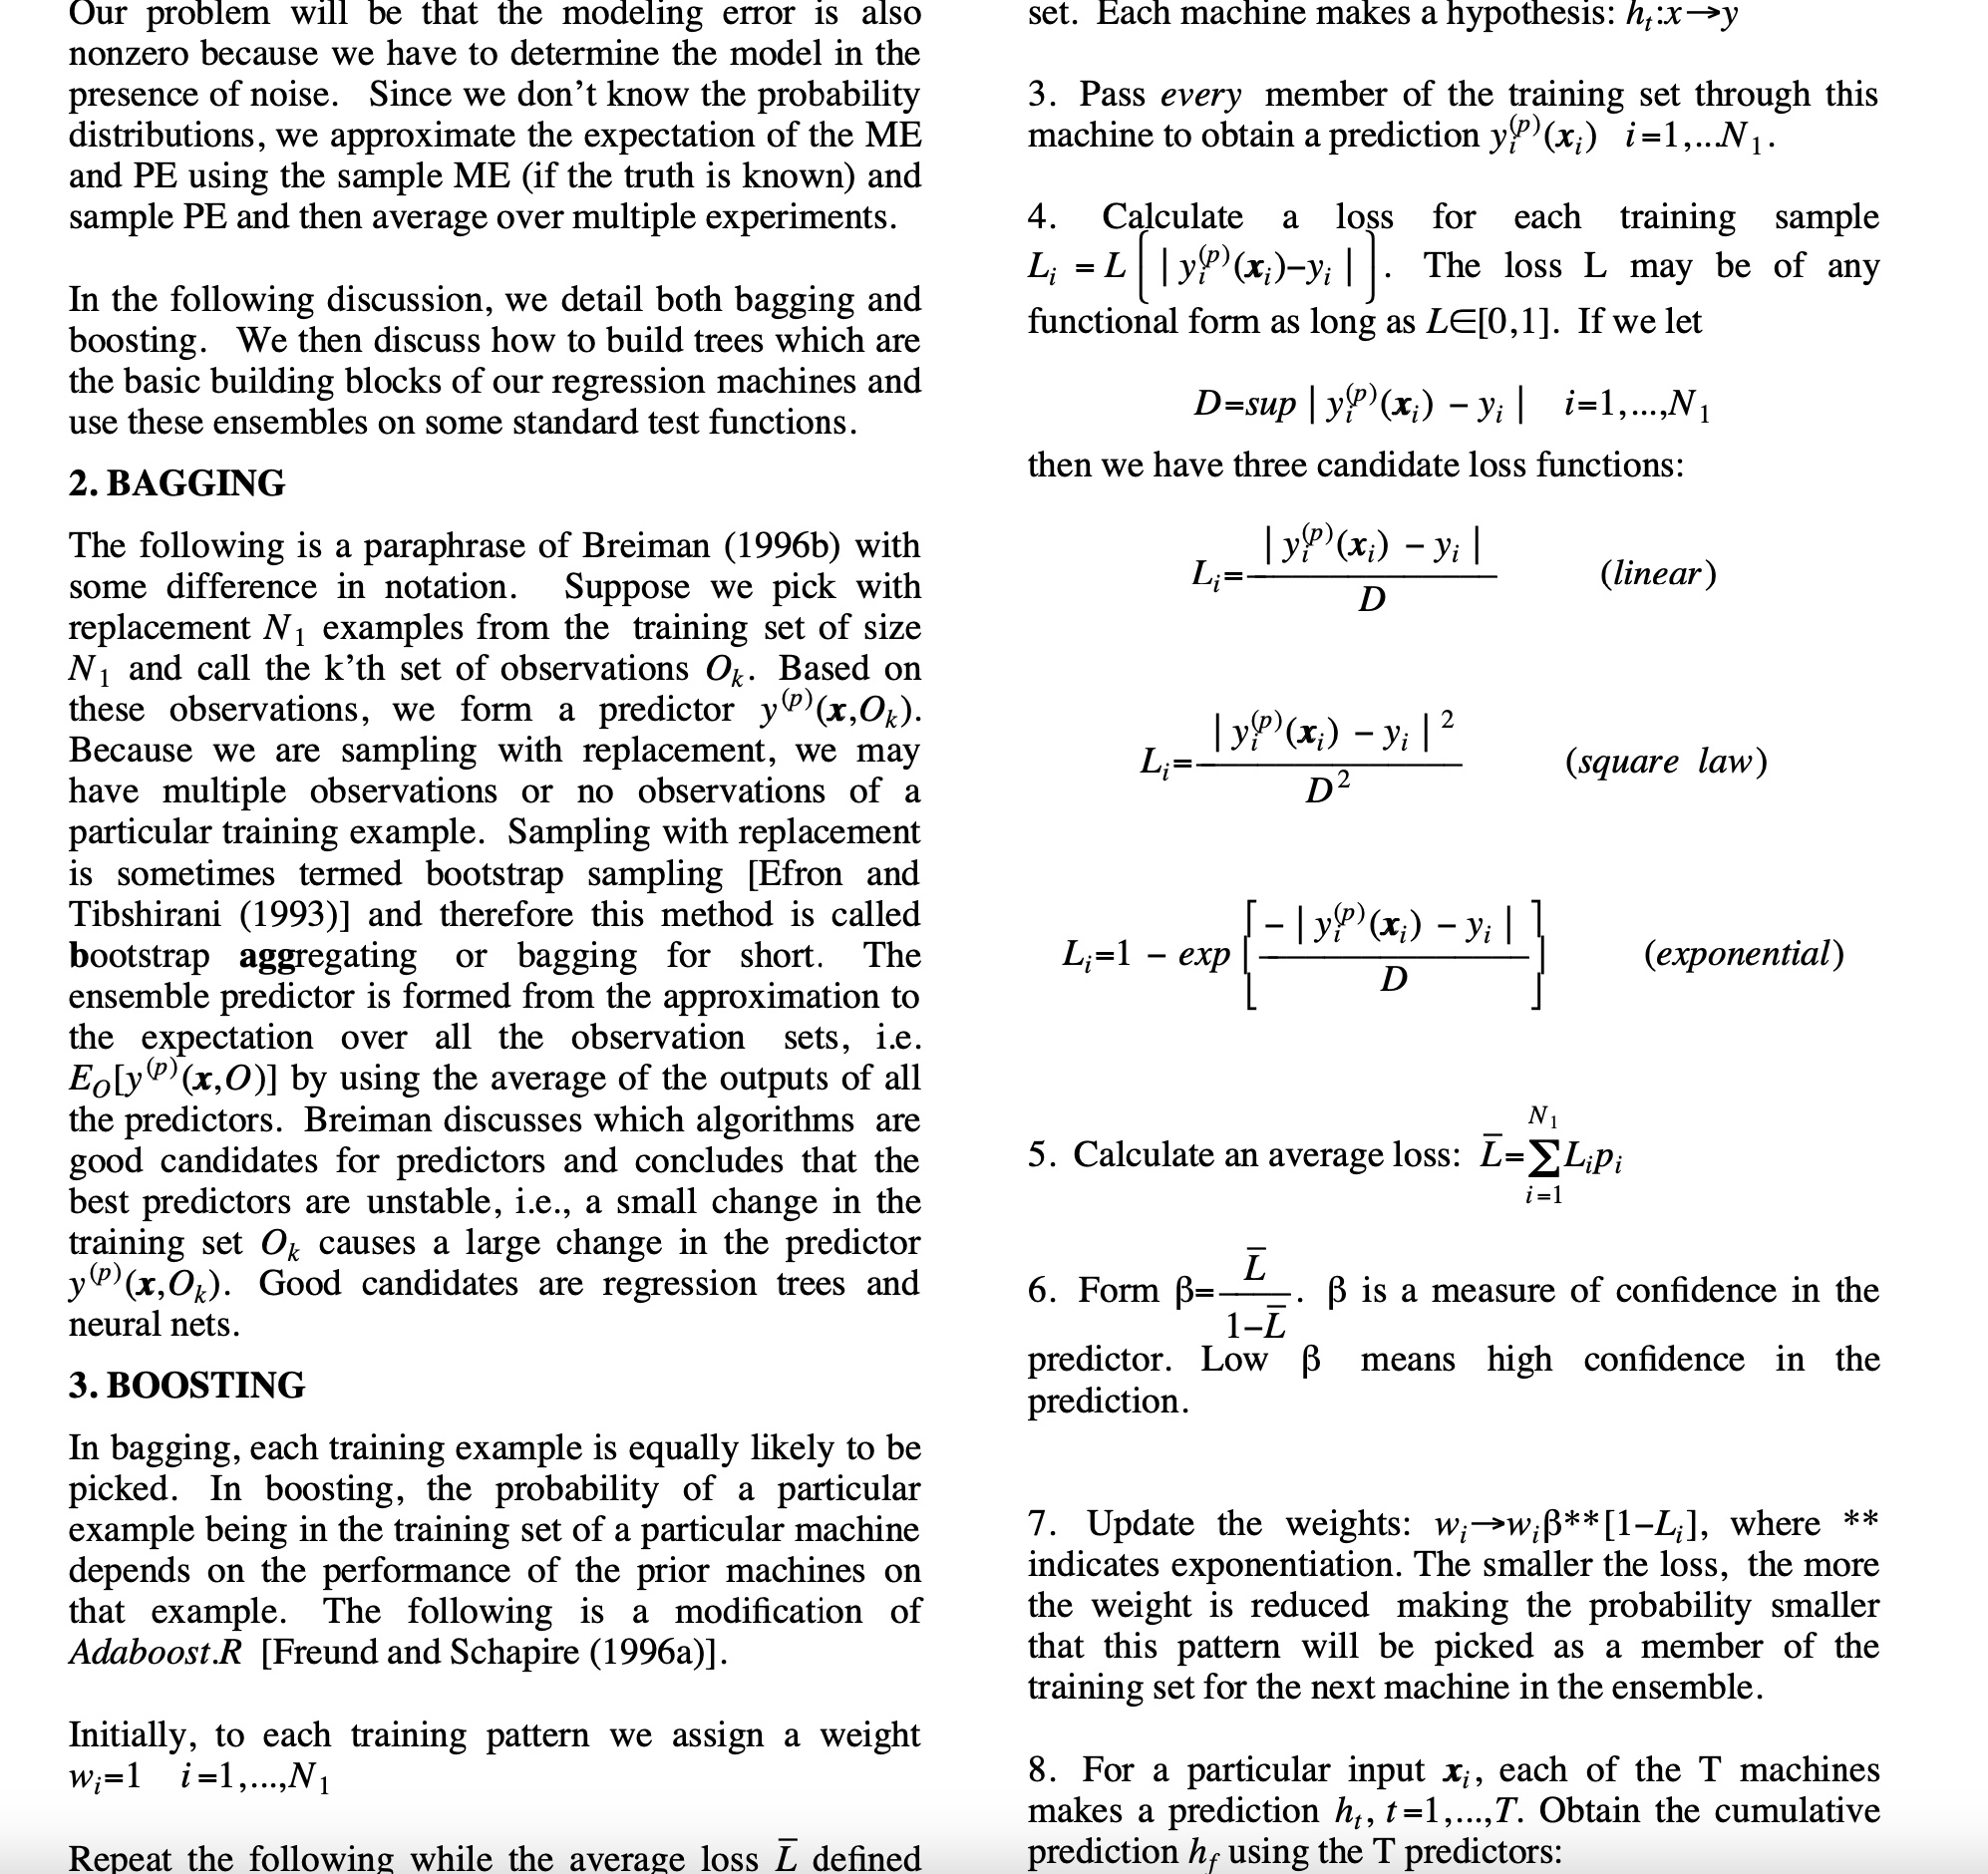
\includegraphics[scale=0.1]{../assets/ensemble/diagrams/adaboost-regression.jpg}}
\end{frame}

\begin{frame}{Random Forest}
  \begin{itemize}
    \item Random Forest is an ensemble of decision trees.
    \item Two types of bagging: bootstrap (on data) and random subspace (on features).
    \item Random feature subsampling decorrelates trees $\Rightarrow$ reduces variance.
  \end{itemize}
\end{frame}

\begin{frame}{Random Forest}
  There are 3 parameters while training a random forest: \textbf{number of trees}, \textbf{number of features (m)}, \textbf{maximum depth}.\\[0.5em]
  \underline{Training Algorithm}\\[-0.2em]
  \begin{itemize}
    \item For $i^{th}$ tree ($i \in \{1 \cdots N\}$), select $n$ samples from total $N$ samples \textbf{with replacement}.
    \item Learn a decision tree on selected samples for the $i^{th}$ round.
  \end{itemize}

  \underline{Learning Decision Tree (for RF)}\\[-0.2em]
  \begin{itemize}
    \item For each split, select $m$ features from total $M$ features and choose the best split only among those $m$.
  \end{itemize}
\end{frame}

\begin{frame}{Dataset}
  \centering
  \fitpic{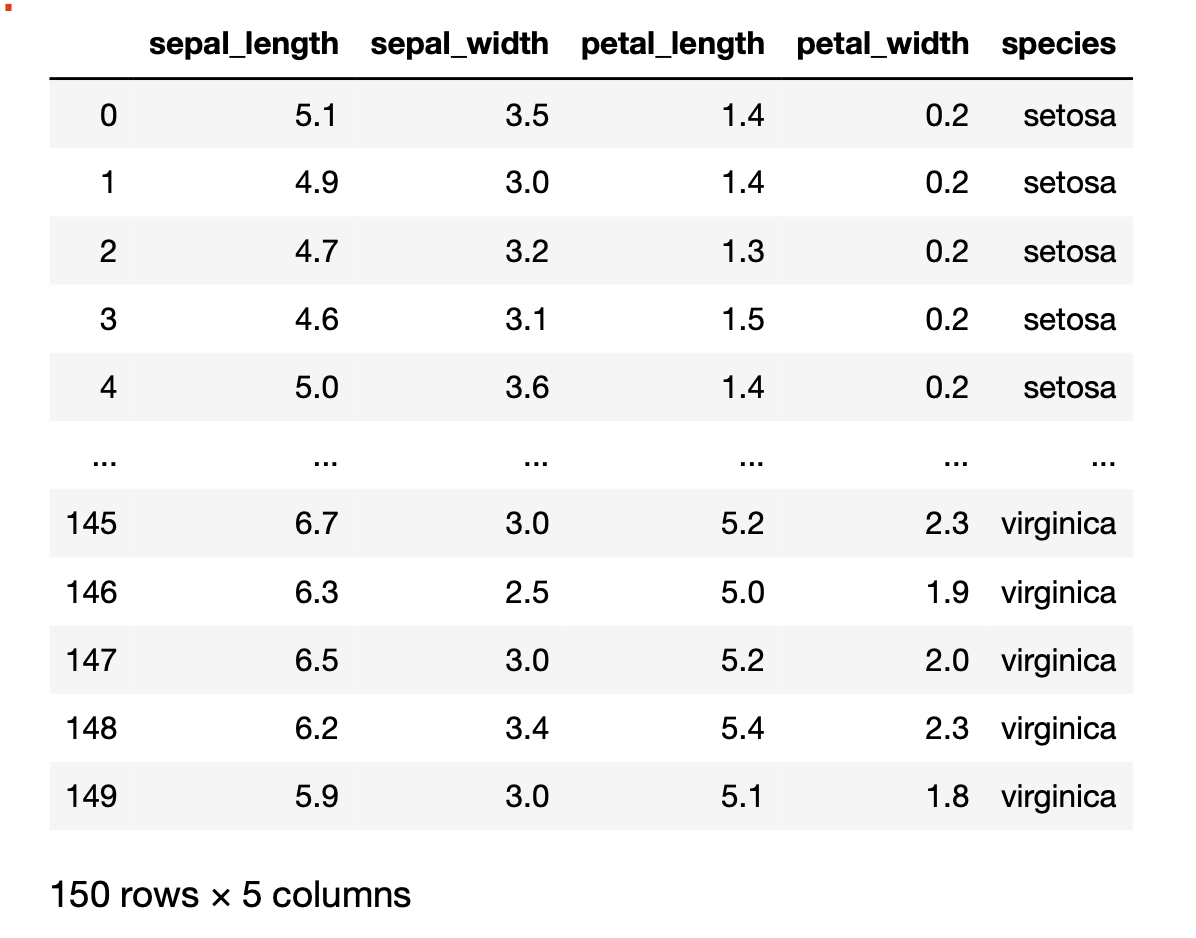
\includegraphics[scale=0.5]{../assets/ensemble/diagrams/dataset-iris.png}}
\end{frame}

% Looping decision tree slides (unchanged content, just fit)
\newcounter{tree}
\forloop{tree}{0}{\value{tree} < 10}{
  \begin{frame}{Decision Tree \# \thetree}
    \begin{figure}\centering
      \begin{notebookbox}{https://nipunbatra.github.io/ml-teaching/notebooks/ensemble-feature-importance.html}
        \fitpic{\includegraphics[scale=0.25]{../assets/ensemble/figures/feature-imp-\thetree.pdf}}
      \end{notebookbox}
    \end{figure}
  \end{frame}
}

\begin{frame}{Feature Importance\footnotemark}
  \centering
  \fitpic{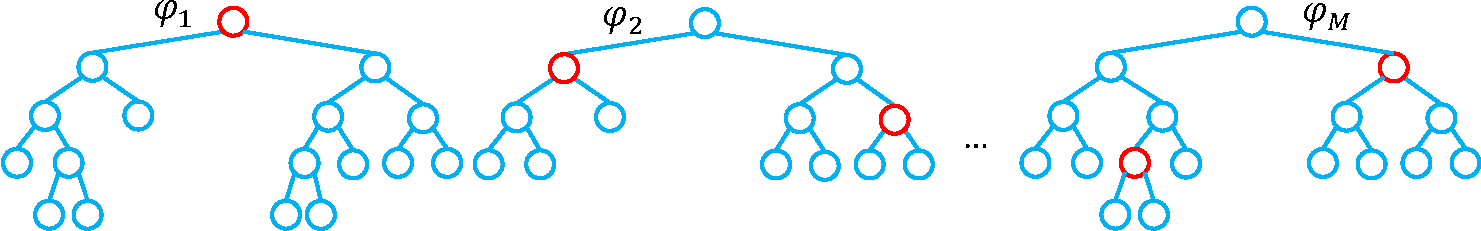
\includegraphics[scale=0.4]{../assets/ensemble/diagrams/mdi.pdf}}
  Importance of variable $X_j$ for an ensemble of $M$ trees $\varphi_{m}$ is:
  \begin{equation*}
    \text{Imp}(X_j) = \frac{1}{M} \sum_{m=1}^M \sum_{t \in \varphi_{m}} 1(j_t = j)\,\Big[ p(t)\,\Delta i(t) \Big],
  \end{equation*}
  where $j_t$ denotes the variable used at node $t$, $p(t)=N_t/N$, and\\
  $\Delta i(t) = i(t) - \frac{N_{t_L}}{N_t} i(t_L) - \frac{N_{t_R}}{N_t} i(t_R)$.
  \footnotetext[1]{Slide Courtesy Gilles Louppe}
\end{frame}

\begin{frame}{Computed Feature Importance}
  \begin{figure}[htp]\centering
    \begin{notebookbox}{https://nipunbatra.github.io/ml-teaching/notebooks/ensemble-feature-importance.html}
      \fitpic{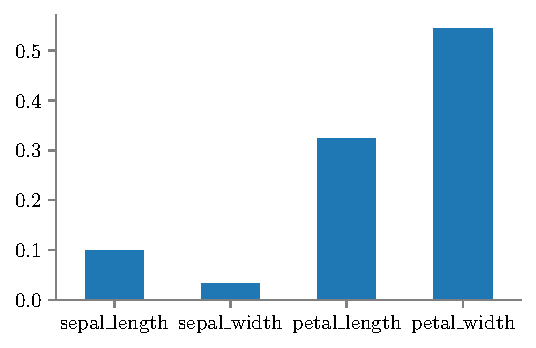
\includegraphics[scale=0.8]{../assets/ensemble/figures/feature-imp-forest.pdf}}
    \end{notebookbox}
  \end{figure}
\end{frame}

\end{document}
